%  The AAU Poster Theme.
%  2013-05-08 v. 1.1.0
%  Copyright 2013 by Jesper Kjær Nielsen <jkn@es.aau.dk>
%
%  This is free software: you can redistribute it and/or modify
%  it under the terms of the GNU General Public License as published by
%  the Free Software Foundation, either version 3 of the License, or
%  (at your option) any later version.
%
%  This is distributed in the hope that it will be useful,
%  but WITHOUT ANY WARRANTY; without even the implied warranty of
%  MERCHANTABILITY or FITNESS FOR A PARTICULAR PURPOSE.  See the
%  GNU General Public License for more details.
%
%  You can find the GNU General Public License at <http://www.gnu.org/licenses/>.
\documentclass[a0paper,portrait]{baposter}
\usepackage{xspace}
\usepackage{xcolor}
\usepackage{xcolor}
\usepackage[utf8]{inputenc}
\usepackage[english]{babel}
%\usepackage{helvet}
\renewcommand{\familydefault}{\sfdefault}
\usepackage[T1]{fontenc}
\usepackage{lipsum}
\usepackage{tabularx}
\usepackage[misc]{ifsym}
\usepackage{fixltx2e}
\usepackage{gensymb}
\usepackage{relsize}

\usepackage{caption}
\captionsetup{
  font=small,% set font size to footnotesize
  labelfont=bf % bold label (e.g., Figure 3.2) font
}

% Make the standard latex tables look so much better
\usepackage{array,booktabs}

% For creating beautiful plots
\usepackage{tikz}
\usetikzlibrary{positioning}
\usetikzlibrary{shapes,arrows,backgrounds,fit,shapes.geometric,calc}
\usetikzlibrary{pgfplots.groupplots}
\usetikzlibrary{patterns}
\usepackage{pgfplots}
\usepackage{pgfplotstable}

\usepackage{amsmath}
\usepackage{amssymb}

% http://en.wikibooks.org/wiki/LaTeX/Colors
\selectcolormodel{RGB}
% define the three aau colors
\definecolor{posterbg}{RGB}{230,230,255}% background colour for the poster

%%%%%%%%%%%%%%%%%%%%%%%%%%%%%%%%%%%%%%%%%%%%%%%%
% Lists
% http://en.wikibooks.org/wiki/LaTeX/List_Structures
%%%%%%%%%%%%%%%%%%%%%%%%%%%%%%%%%%%%%%%%%%%%%%%%
% Easier configuration of lists
\usepackage{enumitem}
%configure itemize
\setlist{%
  topsep=3pt,% set space before and after list
  noitemsep,% remove space between items
  labelindent=\parindent,% set the label indentation to the paragraph indentation
  leftmargin=*,% remove the left margin
  font=\color{black}\normalfont, %set the colour of all bullets, numbers and descriptions to aaublue1
}
\setdescription{font=\color{blue!50!black}\normalfont\bfseries}

%%%%%%%%%%%%%%%%%%%%%%%%%%%%%%%%%%%%%%%%%%%%%%%%
% Misc
%%%%%%%%%%%%%%%%%%%%%%%%%%%%%%%%%%%%%%%%%%%%%%%%
% change/remove some names
\addto{\captionsenglish}{
  %remove the title of the bibliograhpy
  \renewcommand{\refname}{\vspace{-0.7em}}
  %change Figure to Fig. in figure captions
  \renewcommand{\figurename}{Fig.}
}
% create links
\usepackage{url}
%note that the hyperref package is currently incompatible with the baposter class

%%%%%%%%%%%%%%%%%%%%%%%%%%%%%%%%%%%%%%%%%%%%%%%%
% Macros
%%%%%%%%%%%%%%%%%%%%%%%%%%%%%%%%%%%%%%%%%%%%%%%%
\newcommand{\todo}[1]{{\color{red}#1}}
\newcommand{\hilight}[1]{{\color{blue}\textbf #1}}
\newcommand{\arbor}{{\textcolor{blue!30!black}{Arbor}}\xspace}
\newcommand{\julich}{J\"ulich\xspace}
\newcommand{\tb}[1]{\textbf{\textcolor{blue!50!red}{#1}}\xspace}
\newcommand{\centerheader}[1]{\begin{center}\bfseries\Large{#1}\end{center} \vspace{-6pt}}
\newcommand{\imageheader}[1]{\begin{center}\bfseries\large{#1}\end{center} \vspace{-2pt}}

\newcommand{\newemph}[1]{{\color{blue}\em #1}}

\pgfplotsset{every tick label/.append style={font=\footnotesize}}

%%%%%%%%%%%%%%%%%%%%%%%%%%%%%%%%%%%%%%%%%%%%%%%%
% Document Start 
%%%%%%%%%%%%%%%%%%%%%%%%%%%%%%%%%%%%%%%%%%%%%%%%
\begin{document}
%%%%%%%%%%%%%%%%%%%%%%%%%%%%%%%%%%%%%%%%%%%%%%%%
% Some changes that cannot be made in the preamble
%%%%%%%%%%%%%%%%%%%%%%%%%%%%%%%%%%%%%%%%%%%%%%%%
% set the background of the poster
\background{
  \begin{tikzpicture}[remember picture,overlay]%
    %the poster background color
    \fill[fill=white] (current page.north west) rectangle (current page.south east);

    %the header
    \fill [fill=white] (current page.north west) rectangle ([yshift=-\headerheight] current page.north east);
  \end{tikzpicture}
}
% if you want to reduce the space before and after equations, use and adjust
% the following lines
%\addtolength{\abovedisplayskip}{-2mm}
%\addtolength{\belowdisplayskip}{-2mm}

%%%%%%%%%%%%%%%%%%%%%%%%%%%%%%%%%%%%%%%%%%%%%%%%
% General poster setup
%%%%%%%%%%%%%%%%%%%%%%%%%%%%%%%%%%%%%%%%%%%%%%%%
\begin{poster}{
    %general options for the poster
    grid=false,
    columns=3,
    % these two control space between and padding inside
    % the poster boxes
    colspacing=3mm,
    boxpadding=2mm,
    %
    headerheight=0.1\textheight,
    background=user,
    headerborder=closed,
    borderColor=blue!40!black,
    headershape=rectangle,
    headershade=plain,
    headerColorOne=blue!15,
    textborder=rectangle,
    boxshade=plain,
    boxColorOne=white,
    headerFontColor=black,
    headerfont=\Large\sf,
    linewidth=1pt
}

%the Eye Catcher (the logo on the left)
{
  \begin{tikzpicture}[remember picture, overlay]
    \node [anchor=north west,xshift=0.02\paperwidth,yshift=-0.03\headerheight] at (current page.north west) {
      
\includegraphics[height=0.4\headerheight]{HBP_logo.jpg}
    };
    \node [anchor=north west,xshift=0.32\paperwidth,yshift=-0.10\headerheight] at (current page.north west) {
      
\includegraphics[height=0.25\headerheight]{julich_logo.pdf}
    };
    \node [anchor=north west,xshift=0.45\paperwidth,yshift=-0.10\headerheight] at (current page.north west) {
      
\includegraphics[height=0.27\headerheight]{bsc_logo.pdf}
    };
    \node [anchor=north west,xshift=0.61\paperwidth,yshift=-0.10\headerheight] at (current page.north west) {
      
\includegraphics[height=0.25\headerheight]{cscs_logo.pdf}
    };
    \node[anchor=north west,xshift=0.8\paperwidth,yshift=-0.05\headerheight] at (current page.north west) {
      
\includegraphics[height=0.4\headerheight]{images/eu_logo.png}
    };
  \end{tikzpicture}
  \vspace{0.3\headerheight}
}
%the poster title
{ \Huge
  \textbf{\arbor} \\[0.1\baselineskip]
\large 
  A morphologically detailed neural network simulation library for modern high performance computer architectures \\[0.2\baselineskip]
  \small
    Ben Cumming\textsuperscript{a}, Stuart Yates\textsuperscript{a} , Wouter Klijn\textsuperscript{b}, Alexander Peyser\textsuperscript{b}, Vasileios Karakasis\textsuperscript{a}, Ivan Martinez Perez\textsuperscript{c}\\
    \textsuperscript{a}Swiss National Supercomputing Center \hspace{2mm}\textsuperscript{b}
Simulation Lab Neuroscience, IAS, JARA, Forschungszentrum \julich
 \hspace{2mm}\textsuperscript{c}Barcelona Supercomputing Center
}
%the author(s)
{\small
    \vspace{1em} Ben Cumming, \\[0.5em]
    Swiss National Supercomputing Center (CSCS), Switzerland\\
}

%%%%%%%%%%%%%%%%%%%%%%%%%%%%%%%%%%%%%%%%%%%%%%%%
% LEFT HAND SIDE OF POSTER
%%%%%%%%%%%%%%%%%%%%%%%%%%%%%%%%%%%%%%%%%%%%%%%%

%%%%%%%%%%%%%%%%%%%%%%%%%%%%%%%%%%%%%%%%%%%%%%%%
\begin{posterbox}[name=motivation,column=0,row=0,span=2]{Heterogeneous many-core  HPC architectures are the new norm}
    \hfill
    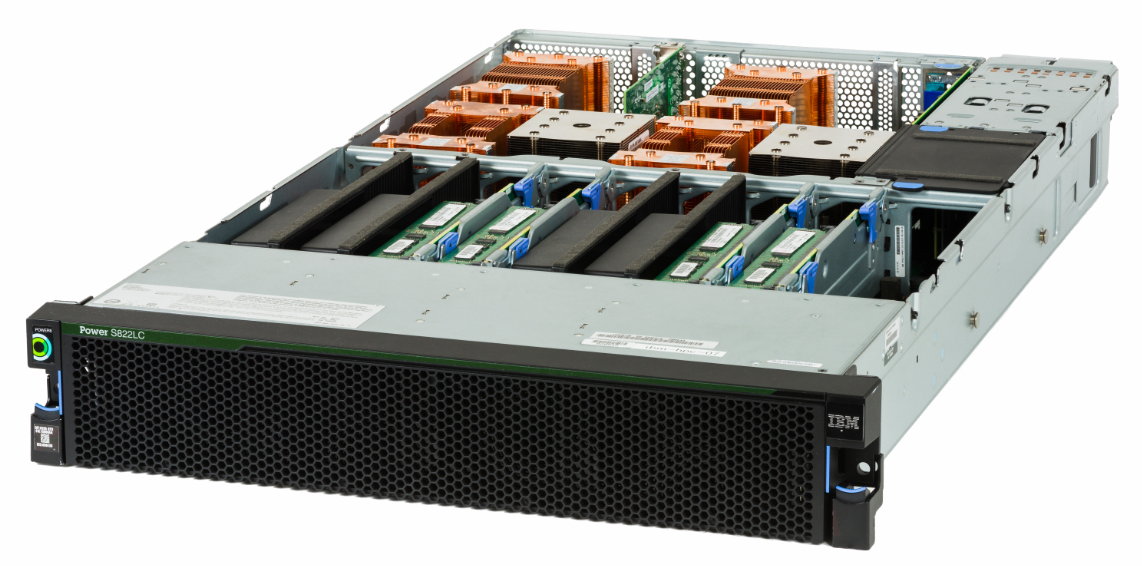
\includegraphics[width=0.35\textwidth]{images/juron.jpg}
    \hfill
    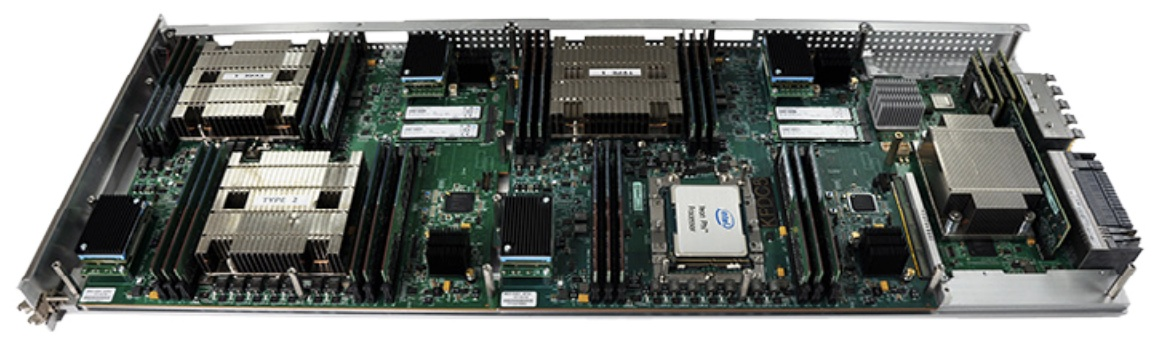
\includegraphics[width=0.55\textwidth]{images/knlnode.jpg}
    \hspace{0.5cm}

    \begin{center}
        The HBP PCP pilot systems at \julich. Both are a radical departure from multicore systems. \\
        \newemph{left}: IBM ``fat node'' with Power8 CPUs and 4 GPUs. \newemph{right}: Cray XC ``blade'' with 4 Intel KNL nodes.
    \end{center}

    These new architectures are already ubiquitous -- we need to develop simulators designed to exploit these architectures now.
    \arbor aims to meet this need, alongside other efforts to add many core support to existing software.
    Designing software from the ground-up for heterogeneous and many-core systems will pay off in the medium to long term.
    \vspace{2pt}
\end{posterbox}
%%%%%%%%%%%%%%%%%%%%%%%%%%%%%%%%%%%%%%%%%%%%%%%%

%%%%%%%%%%%%%%%%%%%%%%%%%%%%%%%%%%%%%%%%%%%%%%%%
\begin{posterbox}[name=who,column=0,below=motivation,span=1]{What is \arbor?}
    \begin{center}
        \colorbox{yellow!20}{\arbor is developed by a team from HPC centers:}
    \end{center}
    \vspace{-9pt}
    \begin{itemize}
        \item CSCS, \julich and BSC in \newemph{WP 7.5.4}
        \item Aim is to prepare neuroscience users for new HPC architectures
    \end{itemize}
    \begin{center}
        \colorbox{yellow!20}{\arbor is designed from the ground up}\\
        \colorbox{yellow!20}{for \newemph{many core}  architectures:}
    \end{center}
    \vspace{-9pt}
    \begin{itemize}
        \item Written in C++11 and CUDA
        \item Using MPI, TBB and C++11 threads
        \item \newemph{Open source} and \newemph{open development}
        \item Sound development practices: \newemph{unit testing}, \newemph{continuous integration}, and \newemph{validation}
    \end{itemize}
    \vspace{-2pt}
\end{posterbox}

\begin{posterbox}[name=progress,column=1,below=motivation,span=1]{Progress \& features}
    \vspace{4pt}
    Highlights of progress since the last HBP Summit:
    \begin{itemize}
        \item Optimized back ends for CUDA, KNL and AVX2
        \item Asynchronous spike exchange that overlaps compute and communication
        \item Efficient sampling of voltage and current on all back ends
        \item Efficient implementation of all features on GPU
        \item Reporting of memory and energy consumption (when available on platform)
        \item An API for addition of new cell types, e.g. LIF neurons and Poisson spike generators
        %\item Kinetic schemes.
        \item Validation tests against numeric/analytic models and NEURON
    \end{itemize}
    
    \vspace{4pt}
\end{posterbox}
%%%%%%%%%%%%%%%%%%%%%%%%%%%%%%%%%%%%%%%%%%%%%%%%

%%%%%%%%%%%%%%%%%%%%%%%%%%%%%%%%%%%%%%%%%%%%%%%%
\begin{posterbox}[name=network,below=progress,column=0,row=0,span=2]{Parallel model and network construction}
    \begin{minipage}[t]{0.5\textwidth}
    \vspace{-4pt}
        In \arbor models are described by \newemph{recipes}:
    \begin{itemize}
        \item Provide a functional model description
        \item Lazy generation of cell attributes to be processed in parallel by a load balancer
        \item Work and memory requirements per node are proportional to cells-per node
        \item Low resource requirements mean model building and simulation need not be separated
    \end{itemize}

   \end{minipage}
    \hspace{10pt}
    \begin{minipage}[t]{0.5\textwidth}
        \begin{center}
            \textbf{Time to build model (20'600 cells/node)}
        \end{center}
        \vspace{-10pt}
        \tikzset{>=stealth', pil/.style={ ->, color=black!60, thick, } }
\begin{tikzpicture}
\begin{semilogxaxis}[
    height=0.7\textwidth,
    width=\textwidth,
    xmin=1,xmax=16384,
    ymin=3.0,ymax=4.5,
    ytick={3, 3.5, 4, 4.5},
    yticklabels={3, 3.5, 4, },
    %axis y discontinuity=crunch,
    xtick={1, 2, 4, 8, 16, 32, 64, 128, 256, 512, 1024, 2048, 4096, 8192, 16384},
    xticklabels={1, , 4, , 16, , 64, , 256, , 1024, , 4096, , 16384, },
    ylabel=\footnotesize time (s),
    xlabel=\footnotesize nodes,
    xticklabel style={yshift=-2pt},
    yticklabel style={xshift=-2pt},
    xlabel style={yshift=7pt},
    ylabel style={yshift=-20pt},
    line width=1.2pt,
    legend style = {at={(1,0)}, anchor=south east},
    grid=major]

    \addplot[color=red, mark=o,mark size=2, only marks, very thick]
        table[x=nodes,y=mpi]
        {images/network-weak.tbl};
    \addplot[color=blue, mark=o,mark size=1, very thick]
        table[x=nodes,y=dry]
        {images/network-weak.tbl};
    \legend{\footnotesize MPI, \footnotesize dry run};

    \node[above, fill=blue!15, align=center, inner sep=1mm]
       (n1) at (axis cs:4,3.25){\scriptsize 21.6k cells};
    \path[pil,->] (n1.north) edge (axis cs:1.1,3.75);

    \node[above, fill=blue!15, align=center, inner sep=1mm]
       (n64) at (axis cs:64,3.5){\scriptsize 1.3M cells};
    \path[pil,->] (n64.north) edge (axis cs:64,4.1);

    \node[above, fill=blue!15, align=center, inner sep=1mm]
       (n16k) at (axis cs:4096,3.6){\scriptsize 353M cells};
    \path[pil,->] (n16k.north) edge (axis cs:15500,4.17);
\end{semilogxaxis}

\end{tikzpicture}

   \end{minipage}
\end{posterbox}
%%%%%%%%%%%%%%%%%%%%%%%%%%%%%%%%%%%%%%%%%%%%%%%%

%%%%%%%%%%%%%%%%%%%%%%%%%%%%%%%%%%%%%%%%%%%%%%%%
\begin{posterbox}[name=targets,column=0,below=network,span=1]{Code generation}
    \vspace{4pt}
    \newemph{Performance portability} presents two challenges:
    \begin{enumerate}
        \item Efficient cell state integration requires hardware-specific implementations
        \item Extensibility demands that new ion channels or synapse models can be provided by simulator users
    \end{enumerate}

    %It is not practical to implement optimized code for each possible mechanism on each platform.\\ \vspace{10pt}

    \vspace{5pt}
    \newemph{Solution}: Use NMODL to describe mathematics and generate optimized code from that for each platform
    \\%\vspace{5pt}

    \vspace{-16pt}
    \begin{center}
      \colorbox{yellow!20}{Current backends}
    \end{center}
    \vspace{-4pt}
    CUDA (NVIDA), AVX512 (KNL \& Sky Lake), AVX2 (Haswell \& Broadwell) and generic C++

    \vspace{4pt}
    Key hardware-specific features:
    \begin{itemize}
        \item \newemph{CUDA} fast key-value reduction for synapse current collection
        \item \newemph{AVX2} vectorised transcendentals for GCC and Clang
        \item \newemph{AVX512} vectorised gather and scatter for per-compartment loads \& stores
    \end{itemize}

    \vspace{17pt}
\end{posterbox}
%%%%%%%%%%%%%%%%%%%%%%%%%%%%%%%%%%%%%%%%%%%%%%%%

%%%%%%%%%%%%%%%%%%%%%%%%%%%%%%%%%%%%%%%%%%%%%%%%
\begin{posterbox}[name=resources,column=1,below=network,span=1]{Resource consumption}
    \vspace{4pt}
    The resources used by a simulation can be measured in different ways:
    \begin{itemize}
        \item \newemph{Time to solution (TTS)}: wall time (s)
        \item \newemph{Node hours (NH)}: $\text{TTS}\times\text{nodes}/3600$
        \item \newemph{Energy to solution (ETS)}: total energy (kJ)
    \end{itemize}

    \begin{center}
        \textbf{Resource consumption for 590k cells.}\\\vspace{3pt}
        \footnotesize
    \begin{tabular}{|l|rrr|rrr|}
        \cline{2-7}
         \multicolumn{1}{ c }{}
        & \multicolumn{3}{ |c| }{daint-mc} & \multicolumn{3}{ c| }{daint-gpu} \\
        \hline
        nodes  & TTS     & NH   &  ETS   & TTS   & NH      &  ETS\rule{0pt}{2.5ex}\\
        \hline
           32  &   204.0 & 1.81 & 1771 & 176.0 &\tb{1.56}&\rule{0pt}{2.5ex}\tb{1159}\\
           64  &   102.4 & 1.82 & 1769 &  89.8 &    1.60 &    1169  \\
          128  &    51.7 & 1.84 & 1743 &  47.1 &    1.67 &    1194  \\
          256  &    26.8 & 1.91 & 1742 &  25.5 &    1.82 &    1247  \\
          512  &\tb{13.5}& 1.91 & 1698 &  15.1 &    2.15 &    1374  \\
        \hline
    \end{tabular}
    \end{center}
    \vspace{-8pt}
        {\tiny\hfill Resource measurements for strong scaling described in ``Performance'' section}\\
    \vspace{-10pt}

    \begin{itemize}
        \item GPU maximises user allocation (86\% NH required to run on CPU)
        \item The GPU uses 65\% energy to solution
        \item CPU can be used when reducing time to solution is most important
    \end{itemize}
    \vspace{4pt}

    \arbor provides good performance on both systems, meeting our \newemph{performance portability} requirement.

    \vspace{8pt}
\end{posterbox}
%%%%%%%%%%%%%%%%%%%%%%%%%%%%%%%%%%%%%%%%%%%%%%%%


%%%%%%%%%%%%%%%%%%%%%%%%%%%%%%%%%%%%%%%%%%%%%%%%
% RIGHT HAND SIDE OF POSTER
%%%%%%%%%%%%%%%%%%%%%%%%%%%%%%%%%%%%%%%%%%%%%%%%

%%%%%%%%%%%%%%%%%%%%%%%%%%%%%%%%%%%%%%%%%%%%%%%%
\begin{posterbox}[name=plots,column=2,row=0,span=1]{Performance}
    {
        \tiny
        \colorbox[HTML]{FCF3CF}{%
            \begin{tabularx}{0.95\textwidth}{l|X}
          daint-mc  & Cray XC40: 2$\times$ 18-core Broadwell per node\smallskip\\
          daint-gpu & Cray XC50: 1$\times$P100 GPU per node\smallskip\\
              cells & 50 compartments \& 5000 synapses per cell\\
                    & Passive dendrites, Hodgkin-Huxley soma\smallskip\\
            network & random\smallskip\\
           duration & 200\,ms\\
            \end{tabularx}
        }
    }
    \vskip4pt
    \imageheader{Strong Scaling}
    \tikzset{>=stealth', pil/.style={ ->, color=black!60, thick, } }
\begin{tikzpicture}
    \begin{loglogaxis}[
        height=0.7\textwidth,
        width=\textwidth,
        xmin=1,xmax=512,
        ymin=1, ymax=256,
        xtick={1, 2, 4, 8, 16, 32, 64, 128, 256, 512},
        xticklabels={1, 2, 4, 8, 16, 32, 64, 128, 256, 512},
        %ytick={1,10,100,200},
        ytick={1, 2, 4, 8, 16, 32, 64, 128, 256},
        yticklabels={1,  , 4,  , 16,   , 64, , 256},
        %yticklabels={1,10,100,200},
        ylabel=wall time (s),
        xlabel=nodes,
        xticklabel style={yshift=-2pt},
        yticklabel style={xshift=-2pt},
        legend style = {at={(0,0)}, anchor=south west},
        line width=1.2pt,
        every axis y label/.style=
            {at={(ticklabel cs:0.5)},rotate=90,anchor=near ticklabel},
        grid=major]

        \addplot[color=red, mark=*, mark size=1.5, mark options={fill=white}]
            table[x=nodes,y=gpusmallt] {./images/strong.tbl};
        \addplot[color=blue, mark=triangle*, mark size=1.5, mark options={fill=white}]
            table[x=nodes,y=mcsmallt] {./images/strong.tbl};

        \node[above, fill=red!15, align=center, inner sep=1mm]
           (gsmall) at (axis cs:1.6,40){\tiny 174 s};
        \path[pil,->] (gsmall.north) edge (axis cs:1.05,150);
        \node[above, fill=blue!15, align=center, inner sep=1mm]
           (msmall) at (axis cs:4,128){\tiny 211 s};
        \path[pil,->] (msmall.west) edge (axis cs:1.1,210);

        \node[above, fill=red!15, align=center, inner sep=1mm]
           (gmin) at (axis cs:280,4){\tiny 5.1 s};
        \path[pil,->] (gmin.west) edge (axis cs:140,5);
        \node[above, fill=blue!15, align=center, inner sep=1mm]
           (mmin) at (axis cs:280,1.7){\tiny 2.2 s};
        \path[pil,->] (mmin.west) edge (axis cs:140,2.2);

        \addplot[color=red!40, mark=*, mark size=1.5, mark options={fill=white, solid}]
            table[x=nodes,y=gpubigt] {./images/strong.tbl};
        \addplot[color=blue!40, mark=triangle*, mark size=1.5, mark options={fill=white}]
            table[x=nodes,y=mcbigt] {./images/strong.tbl};

        \node[above, fill=red!15, align=center, inner sep=1mm]
           (glarge) at (axis cs:32,40){\tiny 176 s};
        \path[pil,->] (glarge.north) edge (axis cs:32,155);
        \node[above, fill=blue!15, align=center, inner sep=1mm]
           (mslarge) at (axis cs:128,140){\tiny 204 s};
        \path[pil,->] (mslarge.west) edge (axis cs:35,210);

        \legend{ {\scriptsize gpu 18k},
                 {\scriptsize mc 18k},
                 {\scriptsize gpu 590k},
                 {\scriptsize mc 590k}
               };
    \end{loglogaxis}
\end{tikzpicture}

    \vskip4pt
    { \small
    Time to solution on CPU and GPU for models with 18'000 and 590'000 cells. GPU performance is better in "throughput mode", i.e. with more cells per node, while CPU is faster with fewer cells per node.
    }

    \imageheader{Weak Scaling}
    \tikzset{>=stealth', pil/.style={ ->, color=black!60, thick, } }
\begin{tikzpicture}
    \begin{semilogxaxis}[
        height=0.7\textwidth,
        width=\textwidth,
        xmin=1,xmax=256,
        ymin=240,ymax=280,
        axis y discontinuity=crunch,
        xtick={1, 2, 4, 8, 16, 32, 64, 128, 256},
        xticklabels={1, 2, 4, 8, 16, 32, 64, 128, 256},
        ytick={250,255,260,265,270,275},
        yticklabels={{~~~250},255,260,265,270,275},
        %yticklabels={50k,100k,150k,200k,250k,300k,350k,400k},
        ylabel=wall time (s),
        xlabel=nodes,
        line width=1.2pt,
        xticklabel style={yshift=-2pt},
        yticklabel style={xshift=-2pt},
        legend style = {at={(0,1)}, anchor=north west},
        every axis y label/.style=
            {at={(ticklabel cs:0.5)},rotate=90,anchor=near ticklabel},
        grid=major]
        \addplot[color=blue, mark=*,mark size=1.5, mark options={fill=white}] table[x=nodes,y=256CPR]
            {./images/scaling_nodes_vs_cpn.tbl};
        \node[above, fill=blue!15, text width=2cm, align=center, inner sep=1mm] (a) at (axis cs:80,272.5){\scriptsize 2,359,296 cells};
        \node[above, fill=blue!15, text width=1.4cm, align=center, inner sep=1mm] (b) at (axis cs:4,270){\scriptsize 9,216 cells};
        \path[pil,->] (a.south) edge (axis cs:230,268.5);
        \path[pil,->] (b.south) edge (axis cs:1.05,263.3);
    \end{semilogxaxis}
\end{tikzpicture}

    \vskip4pt
    { \small
    Time to solution with 4000 cells per node, as the number of nodes is increased. Run time increases by less than 25\% when the problem is scaled by 256$\times$. \arbor has a \newemph{dry-run} mode that was used to tune scaling issues with many nodes.
    }
    %\imageheader{Single Node Performance}
    %\tikzset{>=stealth', pil/.style={ ->, color=black!60, thick, } }
\begin{tikzpicture}

    % ENERGY
    \begin{loglogaxis}[
        axis y line*=right,
        height=0.7\textwidth,
        width=\textwidth,
        xmin=100,xmax=25600,
        ymin=0.2,ymax=600,
        ytick={0.1, 1, 10, 100},
        yticklabels={0.1, 1, 10, 100},
        ylabel=ETS (kJ),
        xlabel=cells,
        xticklabel style={yshift=-2pt},
        yticklabel style={xshift=1pt},
        ylabel style={xshift=-10pt},
        legend style = {at={(0,0)}, anchor=south west},
        line width=1.2pt,
        every axis y label/.style=
            {at={(ticklabel cs:0.5)},rotate=90,anchor=near ticklabel}]

        \addplot[color=red, mark=triangle*, dashed, mark size=2, mark options={fill=white}]
            table[x=cells,y=Egpu] {./images/single_node.tbl};
        \addplot[color=blue, mark=triangle*, dashed, mark size=2, mark options={fill=white, solid}]
            table[x=cells,y=Emc]  {./images/single_node.tbl};
    \end{loglogaxis}

    % WALL TIME
    \begin{loglogaxis}[
        axis y line*=left,
        height=0.7\textwidth,
        width=\textwidth,
        xmin=100,xmax=25600,
        ymin=0.5,ymax=400,
        ylabel=wall time (s),
        xlabel=cells,
        xticklabel style={yshift=-2pt},
        yticklabel style={xshift=-2pt},
        legend style = {at={(0,0)}, anchor=south west},
        line width=1.2pt,
        every axis y label/.style=
            {at={(ticklabel cs:0.5)},rotate=90,anchor=near ticklabel}]

        \addplot[color=red, mark=triangle*, mark size=2, mark options={fill=white, solid}]
            table[x=cells,y=Tgpu] {./images/single_node.tbl};
        \addplot[color=blue, mark=triangle*, mark size=2, mark options={fill=white, solid}]
            table[x=cells,y=Tmc]  {./images/single_node.tbl};
    \end{loglogaxis}
\end{tikzpicture}


    %{ \small
    %Some text to describe it here.Some text to describe it here.Some text to describe it here.Some text to describe it here.Some text to describe it here.Some text to describe it here.
    %}

    \imageheader{Optimization: Updating Membrane Currents on GPU}
    \tikzset{>=stealth', pil/.style={ ->, color=black!60, thick, } }
\begin{tikzpicture}
\begin{loglogaxis}[
    height=0.7\textwidth,
    width=\textwidth,
    xmin=1,xmax=1000,
    ymin=50,ymax=1000000,
    ytick={100,10000,1000000},
    yticklabels={100,10000,1000000},
    xtick={1, 10, 100, 1000},
    xticklabels={1, 10, 100, 1000},
    ylabel=time (ms),
    xlabel=synapses per compartment,
    xticklabel style={yshift=-1pt},
    yticklabel style={xshift=-1pt},
    line width=1.2pt,
    xlabel style={yshift=7pt},
    ylabel style={yshift=-5pt},
    legend style = {at={(1,0)}, anchor=south east},
    grid=major]

    \addplot[color=red, mark=*,mark size=1.5, mark options={fill=white}]
        table[x=syncomp,y=atomic64]
        {images/by_key.tbl};
    \addplot[color=blue, mark=*,mark size=1.5, mark options={fill=white}]
        table[x=syncomp,y=shuffle64]
        {images/by_key.tbl};
    \node[above, fill=blue!15, align=center, inner sep=1mm]
       (p1) at (axis cs:10,1200){\tiny 1.7$\times$};
    \node[above, fill=blue!15, align=center, inner sep=1mm]
       (p2) at (axis cs:100,20000){\tiny 2.4$\times$};
    \node[above, fill=blue!15, align=center, inner sep=1mm]
       (p3) at (axis cs:700,40000){\tiny 11.4$\times$};
    \legend{\footnotesize CUDA atomics, \footnotesize reduce-by-key};
    \node[above,scale=0.8] at (axis cs:13,400000) {
      \begin{minipage}{5cm}
        \relsize{-5}
        blue insets: atomics run time / reduce run time
      \end{minipage}
    };

\end{loglogaxis}

\end{tikzpicture}


    { \small
    Time taken to update 10'000 compartments as the number of synapses per compartment varies.
    Race conditions occur when multiple synapses on the same compartment update compartment current simultaneously. \arbor has an optimized reduce-by-key operation that improves performance over naive CUDA atomics when many synapses are attached to the same compartment.
    }
    \vspace{0pt}
\end{posterbox}
%%%%%%%%%%%%%%%%%%%%%%%%%%%%%%%%%%%%%%%%%%%%%%%%
%%%%%%%%%%%%%%%%%%%%%%%%%%%%%%%%%%%%%%%%%%%%%%%%
\begin{posterbox}[name=contact,column=2,below=plots,span=1,headerColorOne=blue!40!black,headerFontColor=white]{Get in touch!}
    \centering
    %The source code is available on GitHub.
    %\newemph{If you would like to know more please contact us!}

    \colorbox[HTML]{FCF3CF}{%
        \begin{tabularx}{0.95\textwidth}{l|X}
            %web   & {eth-cscs.github.io/arbor}\smallskip\\
            source& {github.com/eth-cscs/arbor}\smallskip\\
            email & {bcumming@cscs.ch}\\
                  & {a.peyser@fz-juelich.de}\smallskip\\
        \end{tabularx}
    }
\end{posterbox}
%%%%%%%%%%%%%%%%%%%%%%%%%%%%%%%%%%%%%%%%%%%%%%%%

\end{poster}
\end{document}
